% This example An LaTeX document showing how to use the l3proj class to
% write your report. Use pdflatex and bibtex to process the file, creating 
% a PDF file as output (there is no need to use dvips when using pdflatex).
% Modified 

% This dissertation was built upon base template provided.

\documentclass{l3proj}

\begin{document}

\title{Team I: ResDiary Restaurant Recommendation System}

\author{Vladimir Bardarski \\
        Paulius Dilkas \\
        Domantas Jurkus \\
        Eduard Kalfov \\
        Josh O'brien \\
		Joseph O'Hagan}

\date{31st March 2017}

\maketitle

% ##################################################
% LAST EDIT: 	06/03/17	Joseph
% ##################################################
\begin{abstract}
The abstract shall go here! Here is some things to keep in mind while writing it.
\end{abstract}

\begin{itemize}
\item The abstract is likely the first substantive description of your work read by an examiner. View it as an opportunity to set accurate expectations.
\item The abstract is a summary of the whole thesis. It presents all the major elements of your work in a highly condensed form. (Write it having written the rest of the paper) The paper sets the abstract.
\item It must be capable of substituting for the whole paper when there is insufficient time and space for the full text.
\item Keep it short and snappy. 
\item The primary function of your thesis (and by extension your abstract) is not to tell readers what you did, it is to tell them what you discovered.
\item Approximately the last half of the abstract should be dedicated to summarizing and interpreting your results.
\item The most common error in abstracts is failure to present results.
\end{itemize}

% Comment out this line if you do not wish to give consent for your work to be distributed in electronic format.
% We hereby give consent - spread the knowledge - pending on result of project
\educationalconsent
\newpage

%==============================================================================

% ##################################################
% LAST EDIT: 	06/03/17	Josh
% ##################################################
\section{Introduction}
\label{sec:intro}
% An introduction, explaining the purpose of the document, a very brief outline of the project and a summary of the structure of the rest of the document (approximately 1-2 pages).

The Professional Software Development (PSD3) course at The University of Glasgow requires students to engage with the practices and methodologies used in modern large-scale software engineering. The purpose of this dissertation is to document the development of the software project created as part of this course by Team I. 

% ---------- A ----------
The project was to build, over the course of several months, a recommendation engine for the Glasgow-based company ResDiary.
The main deliverable was a system capable of producing sensible restaurant recommendations for existing ResDiary users; a system that could be integrated into the existing ResDiary platform at a later date. 

Our team consisted of six third-year Computing Science students. Within the group there was a broad range of skills, interests and experience - with two members actively working as software professionals, and another having participated in an internship. For some members, however, this was a first opportunity to interact with a real client. 

In this document we outline, in detail, the entire process: from the initial requirements gathering with our customer, through to final system delivery. 

In section \ref{sec:background} we present the background to the project, the motivations of the customer and how we arrived at the agreed deliverables.

%this will surely be expanded to enumerate each separate section better I would like to discuss in detail the practices, issue-tracking, the team work/team load - Josh etc.

In subsequent sections \ref{sec:alice} through Section \ref{sec:reflections} we explore the challenges we faced through development and the steps we took to resolve them, explore the impact of team dynamics on the outcome and reflect on what we have learned from the experience. We also explain how we applied the good development practices learned in PSD3. In particular we highlight the role of version control, agile development and issue tracking.

\newpage

% ################# Comment Log ####################
% 	A. 	We mention the integration but the final 
%		state of the system is for it to be used
%		as a proof of concept / prototype by RD.		<--	Joseph 
% ##################################################

%==============================================================================

\section{Case Study Background}
\label{sec:background}
% A description of the case study background and context. This should include a description of the project customer (what was the nature of the organisation you were working for), their objectives for the project, and a summary of what was actually achieved. Where appropriate, this section should also make reference to similar related projects in order to make the context clear (approximately 4-5 pages).

% ##################################################
% LAST EDIT: 	15/03/17	Dom
% ##################################################
\subsection{Customer}
\label{sec:customer}
% The customer organisation and background.

% Here we want answer the question of who are ResDiary and what do they do.
% Additionally answer who played the customer role of ResDiary to us on the project.

% Who are ResDiary?
ResDiary are a Glasgow-based online restaurant reservation service; a commercial organisation providing a comprehensive, easy to use booking and table management platform for use by both the hospitality industry and its guests. The company provides 24-hour reservation services via websites including Facebook and Twitter as well as their own booking portal ResDiary.com. Their global service sees 9.7 million covers booked every month and their technology is in use in over 6,500 restaurants across 58 countries.

ResDiary senior software engineers Adam Connelly and Ian Strachan acted as representatives throughout the duration of our project. They served as the point of contact between our team and the customer, providing useful feedback and answers to our queries during development. Most notably, they provided our team with anonymised sample datasets from the ResDiary database which were essential for the project.

% ################# Comment Log ####################
% Mention their names? you sure? - Dom
%	-> Other dissertations did it so sure - Joseph
% Served as SLAVES - Dom
% ##################################################

% ##################################################
% LAST EDIT: 	15/03/17	Joseph
% NOTE: 		Reference papers on Amazon / Netflix Models / Netflix Prize
% ##################################################
\subsection{Customer Objectives And Rationale}
\label{sec:custobjectives}
% The rationale and initial objectives for the project.

% Initial Meeting and the customer's motivation for the project.

The initial customer meeting occurred on October 19th and was led by Ian Strachan. This was our first contact with the customer and served as the customer requirements elicitation meeting. The meeting began with an overview of the ResDairy business \ref{sec:customer} and some information being given of the technologies in place within their system. This included information on the particular development languages being used though the primary reason being to provide the background context for the large quantities of data being gathered by ResDiary from their daily operation. This large mass of big data however is currently unused which the ResDiary developers view as a significant shortcoming of their system. 

As such the company is exploring potential utilisation methods of this vast quantity of data which they believe they will be allow them to distinguish themselves from their competition and gain a commercial edge. Having conducted some research they have discovered that none of their competitors currently offer a restaurant recommendation service within their particular booking platform. ResDiary believe such as system, which would make recommendations to users based off their previous dining habits and similarity to other users, will give them an advantage over their competition. They believe such a feature will increase restaurant discovery on their service which is of benefit to both their customers and the organisation itself.

The inspiration of the idea stems from the similar system provided by services such as Amazon and Netflix (!R! REFERENCE PAPERS ON NETFLIX AND AMAZON RECOMMENDATIONS MODELS !R!). The Netflix model in particular being the closest reference point for the system they wish to replicate due the similarity between making recommendations based on a user’s history and similarity to other users. As a starting point for our own research into creating such a system they suggested looking into the 2009 Netflix Prize competition (!R! REFERENCE SECTION ON RESEARCH INTO SIMILAR SYSTEMS AND HOW WE ARRIVED AT OUR MODEL !!!). The goal of this competition was to produce the best algorithm which could most accurately predict a user’s rating of a film based on previous ratings and no other additional information about the users or the films. This they felt would be a good starting point for the development of such a system.

While the primary focus of our project was to be the development of the recommendation system, time was spent discussing what the customer viewed as the end state of the system, whether it be integration into the existing ResDiary portal or as a proof of concept prototype. As the customer was currently undecided in this regard, partly due to an internal transition in development technologies, they elucidated our initial aim should be to focus on the creation of the recommendation system as the end state was currently susceptible to change. The decision regarding the final state of the project ultimately would not be made until midway through the development cycle (!R! REFERENCE TO FINAL DECISION STATE OF SYSTEM SECTION !R!) when the customer decided to view the project as the latter of the two initially proposed systems.

% ################# Comment Log ####################
% ##################################################

\subsection{Our Initial Objectives}
\label{sec:ourinitobjectives}
% ##################################################
% LAST EDIT:  15/03/17  Joseph
% NOTE:         Needs reworking
% NOTE:			Needs referencing
% NOTE:			Needs cutting down page count 
% ################################################## 

Having conducted the requirements elicitation meeting production began on a requirements specification which would serve as the project proposal document to be presented to the client at the next customer meeting on November 16th. This occurred in tandem with conducting the initial necessary background research necessary for the project (!R! REFERENCE BACKGROUND RESEARCH SUBSECTION !R!) due risks and costs associated with a project of this nature (!R! REFERENCE MINI REFLECTION ON IMPORTANCE OF INITIAL REQUIREMENTS GATHERING !R!). The proposal document included the functional and nonfunctional requirements the team agreed upon based on our interpretation of the customer’s initial pitch of the project. Although these would be continually revised and refined as the project developed it was initially proposed for the project to meet the following functional and nonfunctional requirements:

Initial functional requirements (!!! subsection !!!):
\begin{itemize}
\item The recommendation engine must accurately suggest restaurants based on the user’s dining history and similarity to other users with similar eating preferences.
\item Recommended restaurants should be in close proximity to where the user typically eats or the geographical location of where they are currently searching.
\item The recommendation engine may recommend restaurants the user has previously visited should the user optionally select for this to occur.
\end{itemize}

Initial nonfunctional requirements (!!! subsection !!!):
\begin{itemize}
\item The engine should be written to allow for easy integration into the existing Resdiary system.
\item The system should give a response within 1 second after receiving the request (provided data is stored locally).
\item New users should be presented an optional quick questionnaire to gather initial data.
\item User and restaurant locations should be interpreted using coordinates rather than city  name as those are of arbitrary precision within the dataset.
\end{itemize}

A set of user stories (ranked by priority) which were then subdivided into individual tasks was also provided in addition a proposed high-level system UML diagram (!R! REFERENCE UML DIAGRAM !R!) and a step-by-step workflow of how the system would generate recommendations. Due to the customer’s ambiguity regarding the final state of the system, the proposed endpoint for the system was left intentionally vague to allow for flexibility in the customer’s vision. Instead the emphasis was to build and produce the most accurate recommendation for a given user.

% ################# Comment Log ####################
% If required (page count) maybe cut down requirements engineering and incorporating customer feedback in reflection point - we did it pretty well though there isn't much to improve in that regard
% ##################################################

\subsection{Customer Refinements To Initial Objectives}
\label{sec:custrefineinitobj}
% ##################################################
% LAST EDIT:  15/03/17  Joseph
% NOTE:         Needs reworking
% NOTE:			Needs referencing
% NOTE:			Needs cutting down page count 
% ##################################################

% The suggested alternative was to use a nightly build system which the team would utilise in the final version of the system (!R! REFERENCE TO SPARK REFLECTION !R!).

Presenting our proposal to the customer, they felt we had a good grasp of their vision as they agreed with the proposed functional requirements and could envision how our high level system would operate and integrate into their existing one. In particular they expressed interest in the potential to “fine tune” the system through altering the significance place on individual recommenders. Concern was expressed though with the (!!! proposed response rate / local computation of recommendations !!!) as the customer felt the need to further clarify the volume of data the system would be expected to work with in a real world deployment. The suggested alternative was to use a nightly build system as this was their expected from the system would operate under in a real world setting. In addition they suggested developing a lightweight front end application to display the recommendations. They rationalised its throwaway nature with the with the belief that such an application would help them to better understand the system, assist with demonstrating the functionality of the system and provide a clear indication of if the system could produce sensible results. 

Incorporating this this feedback into the specification  the team felt the need to revise the nonfunctional requirements of the project. This saw the removal of the aforementioned “1 second local response rate” (!R! REFERENCE ORIGINAL NONFUNCTIONAL REQUIREMENTS !R!) in place of the following two requirements:

\begin{itemize}
\item Provided the data is not stored locally, the system should be setup to allow for nightly updates to the recommendations made.
\item Have the ability to “fine tune” the recommendation engine by altering the weighting significance of different components of the recommendation such as distance, price, 
reviews, etc.
\end{itemize}

Furthermore a soft goal developed within the team to produce a front end application to showcase the recommendation system. While some of the team felt this justified being defined within the specification the majority instead felt the focus of the project should be on creating the most accurate recommendations and delay defining an end state until it was defined by the customer. Should the customer not provide clarity earlier it was decided to press for clarity on this issue during the scheduled January 26th meeting and define a agreed handover state for the project.

Prior to the January meeting the development efforts were split between the creation of this throwaway application and on the long term solution to the problem. The prototype system was also used during an interim meeting on December 7th where the technical decisions of the long term solution discussed at length as they were being finalised and implementation of them commenced (!R! REFERENCE TECHNICAL REFLECTIONS !R!).  

% ################# Comment Log ####################
% If required (page count) maybe cut down requirements engineering and incorporating customer feedback in reflection point - we did it pretty well though there isn't much to improve in that regard
% ##################################################

% \subsection{Technical Research \& Prototyping}
% \label{sec:techresearchproto}
% ##################################################
% LAST EDIT:  15/03/17  Joseph
% NOTE:         Perhaps best to merge with above subsection
% ##################################################

% ################# Comment Log ####################
% ##################################################

\subsection{Defined End State of System}
\label{sec:jandefinedstate}
% ##################################################
% LAST EDIT:  15/03/17  Joseph
% NOTE:         Needs reworking
% NOTE:			Needs referencing
% NOTE:			Needs cutting down page count 
% ##################################################

Upon presenting the progress made at the January 26th meeting the team pressed the customer regarding what their vision of the final state of the system. Through this discussion it became clear the customer wished to view the project as “proof-of-concept” with their intended use being to assess the worth of creating a similar system for their existing system. Additionally they wished to learn from the system, as they have little experience in this particular field, and should they believe a similar system to be of use to their business they wished to use our system as a prototype to justify the development resources required. 

With the final handover state of the system known, the team decided a redesign of the front end of the application was necessary. (!R! TIE IN / REFERENCE BENEFITS OF STARTING AFRESH !R!). The primary justification for the redesign coming through an observation made while giving the demonstration at the January 26th meeting to a non-technical member of the ResDiary team. Through this non-technical perspective it was clear that the system was not properly communicating the recommendations being made as it was unclear to a non-technical user how the system generally operated, if it was functioning correctly and if the results it produced were sensible. As the end state of the system was now clearly defined end state the following functional requirements were discovered and added to the project with the aim of producing a front end redesign which visually showed the system was operating correctly and producing accurate predictions:

Functional
\begin{itemize}
\item The front end display should display recommendations for a random pool of users to simulate typical use of the system.
\end{itemize}

Nonfunctional
\begin{itemize}
\item The front end be designed such that it is aesthetically clear that the recommendations made are sensible and accurate.
\end{itemize}

With the addition of the above requirements the decision was made in the aftermath of the January 26th meeting to drop the proposed nonfunctional requirement of implementing recommendations for new users. A more detailed account into this decision can be found in Section (!R! REFERENCE DROPPED FEATURE REFLECTION POINT !R!) though the general belief was that such a feature was of particular interest to the customer and thus should be dropped from the intended implementation of the project.

% ################# Comment Log ####################
% ##################################################

% ##################################################
% LAST EDIT: 	06/03/17	Joseph
% ##################################################
\subsection{Delivered Software}
\label{sec:finsoftware}
% Information on the final software that was delivered to the customer.
This section can only be written after the software is in its final handover state.
\newpage

% ################# Comment Log ####################
% ##################################################

%==============================================================================
\section{Alice}
\label{sec:alice}

This is a example of how to include an image from the figures directory.

\begin{figure}
\begin{center}
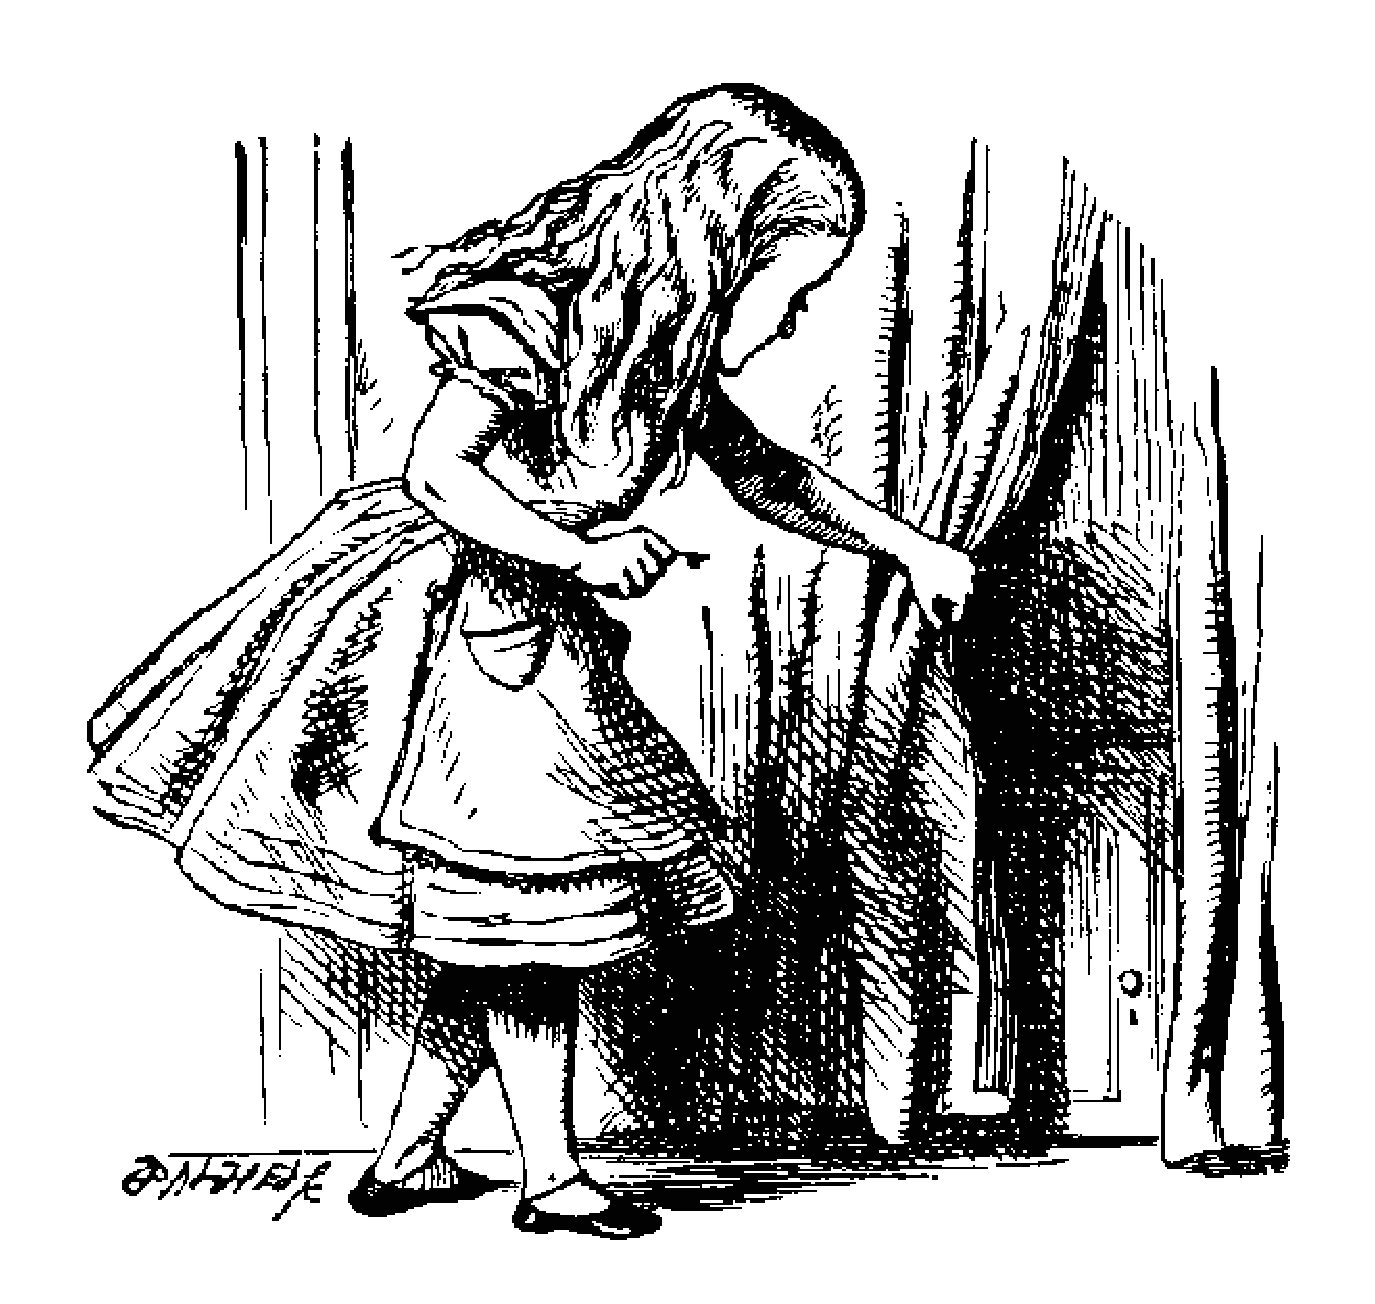
\includegraphics[width=7cm]{figures/alice}
\end{center}
\caption{Behind it was a little door}
\label{fig:alice}
\end{figure}

This is an example of how to reference an inlcuded figure (see Figure \ref{fig:alice}).

%==============================================================================
\section{Reflections}
\label{sec:reflections}
% ##################################################
% LAST EDIT: 	14/03/17	Joseph
% NOTE:	Currently misc. thoughts / notes
% ##################################################

% Several sections that reflect on your experiences during the team project. Each section should discuss one theme, characterised by incidents or events that occurred during the team course of the project from which you learned (approximately 12-15 pages).

As for the general structure of Section 3 the way I envision it. Regarding the order I envision starting by saying the team utilised Scrum and then reflect on whether Scrum was the right choice for the final reflection point / conclusion. The order of the other points can be changed around for best flow:
\begin{itemize}
\item SCRUM Overview - start with an overview stating the team used Scrum and maybe a brief sprint summary with reflection references or mini-reflections. The sprint summary may not be necessary as a good deal of context is provided above in relation to the development of the project.
\item Technical Decisions - this will be three sub reflections regarding 1. Choice of language 2. Choice of collab / content models 3. Choice of Spark
\item Testing - a section on testing and whether a better testing strategy could have been used.
\item Dropped Features - features were dropped and this raises the question why? So of the reasons were our own fault and some were not. This is worth hitting on and also provides a transision into reflection on our failures for why the features were cut from the project.
\item Team Structure - this was a significant shift in how the team internally thought of the project and is worth mentioning.
\item Communication and Task Backlog - communication came up again and again in retrospectives and so should feature.
\item Code Reviews - code reviews came up and were the thing our project really lacked as far as markers are concerned. Would also have prevented several issues the team faced during the development process.
\item Scrum vs XP / etc - was using the Scrum system the correct system? This I feel leads naturally into the conclusion from the third section as its a reflection that can tie in the other reflection points as well. Ties them all together and leads out of the reflection section somewhat naturally.
\end{itemize}


Start by stating that the team decided to use the Scrum methodology and reference reflection point of if this was the correct system to use. Potentially give iteration overview (short summary of each iteration) with either a mini-reflection or reference to further reflection point for all key points which occurred.
\begin{itemize}
\item Sprint 1 - importance of getting the requirements correct - risks \& costs of fixing, etc (MINI REFLECTION).
\item Research conducted and technical decisions - reference to reflection points.
\item Dropped Feature - reference to reflection point.
\item Testing - reference to reflection point.
\item Front end redesign - throwaway code and prototyping (MINI REFLECTION)
\item Pair Programming - reference to reflection point 
\item ETC
\item ETC
\end{itemize}

\subsection{FINAL REFLECTION POINT - Scrum vs XP - Was Scrum The Right Choice}
\label{sec:scrumvsxp}
% ##################################################
% LAST EDIT:  15/03/17  Joseph
% NOTE:         Temp notes / thoughts
% ##################################################
This would be a reflection on using the Scrum system in comparison to another system such as Extreme Programming which might have been more suited to our project given its vague nature at the start and would also have helped combat the issues of code reviews / testing.

We ended up with this weird cross system that was mainly Scrum.

Probably pick one then compare against the other and determine if that would have worked better. Probably closer to Scrum of the above two.

Misc points:
\begin{itemize}
\item Time between meetings served as a good sprint dates - working on smaller iterations may have ensured better communication within the team.
\item Development typically did not change much within a sprint - XP difference here may not have made much of a difference though the dropped feature could have been explored earlier in the development cycle than the 2nd semester.
\item Task priority was a bit of an issue as we didn’t really do proper task estimation - XP would have solved that issue as it forces strict policy and task estimation.
\item Scrum has no engineering practices whereas our project definitely should have. XP would have forced pair programming from the start (rather than sporadic occurrences within sprints), ensured better, more thorough testing from an earlier stage in the project and avoided the whole code review “you deleted all my code you bastard” arguments.
\end{itemize}

% ################# Comment Log ####################
% ##################################################


\subsection{REFLECTION POINT - Team Structure}
\label{sec:teamstructure}
% ##################################################
% LAST EDIT:  15/03/17  Joseph
% NOTE:         Temp notes / thoughts
% ##################################################

REFLECTION POINT - Anarchy into Structure (Team Structure)
Initially the team had no real structure and instead utilised a developer anarchy team structure whereby someone would work on whatever system of the felt like at a given time. This eventually stopped working as the team subdivided into divisions - front end, back end and testing with back end being further divided into collaborative filter, evaluator, content based, NEO recommender.

Anarchy would explain the lack of time estimates and product owner however.

Reasons for the failure of the anarchy include the following reasons:

\begin{itemize}
\item Failure to communicate between the team - people weren’t discussing what they were actively working on, tickets didn’t reflect what people were working on, people didn’t yield results in an efficient enough manner.
\item Failure to fully understand domain - anarchy structures require huge expertise of the problem domain which regardless of how smart you are you cannot gain a grasp of in a few weeks. There’s a reason we pay for years worth of experience in a field / industry.
\item Motivation took a hit over Christmas (it was the holidays)
\item Lack of trust between team as this was the first time we worked together as a team on a long term project.
\end{itemize}

Changing to a more structured development system did have an effect on productivity (testing improved - we actually had some, front end redesign was rad, more defined roles resulted in better communication within the team)

% ################# Comment Log ####################
% ##################################################

\subsection{REFLECTION POINT - Code Reviews \& Branching}
\label{sec:codereviewbranch}
% ##################################################
% LAST EDIT:  15/03/17  Joseph
% NOTE:         Temp notes / thoughts
% ##################################################
We did not do code reviews and this resulted in some ‘tensions’ during the development of the project. Code reviews from the start of the development would have been beneficial for many reasons (see papers).

Misc Points:
\begin{itemize}
\item The system was designed such that branching was unnecessary for the project. Branching was somewhat discouraged throughout the project in order to reduce merge costs / time. Whether the time saved outweighs the time spent fixing and altering other people’s code remains to be seen.
\item Lack of code reviews meant that the code often had inconsistent styling.
\item Lack of code reviews meant a significant portion of time was spent fixing or altering other people's code to work with parts of the system they did not realise they had broken.
\item Lack of code reviews meant code which was WIP was deleted prior to it being fully implemented into the system - again lack of branching issue somewhat.
\item Suggested at the first retrospective but ended up avoiding. Would have reduced a number of problems with development cycle but you can't be perfect.
\item Highlighted in retrospective 3 with the code integration being highlighted.
\item Highlighted even more in retrospective 4 with code integration really being highlighted.
\end{itemize}

% ################# Comment Log ####################
% ##################################################

\subsection{REFLECTION POINT - Apache Spark}
\label{sec:sparkreflection}
% ##################################################
% LAST EDIT:  15/03/17  Joseph
% NOTE:         Temp notes / thoughts
% ##################################################
Misc Points:
\begin{itemize}
\item Team decided the entire team should spend time over Christmas playing around with Apache Spark to ensure common understanding of the system between team members. This may not have been the best use of resource and instead team could have split earlier and the front end developers not bothered playing around with it as they did not end up touching it directly during the development of the project. 
\item Common knowledge was gained though but a more typical front end, back end split in focus may have been beneficial and resulted in an improved front end application sooner.
\end{itemize}

% ################# Comment Log ####################
% ##################################################


\subsection{REFLECTION POINT - Dropping Features}
\label{sec:droppingreflection}
% ##################################################
% LAST EDIT:  15/03/17  Joseph
% NOTE:         Temp notes / thoughts
% ##################################################

Misc note from section 2:
While this particular feature had been viewed as a bonus feature from the outset of development the team felt based on the customer’s feedback that the customers were not particularly interested in such a feature. Research conducted earlier had shown that making recommendations of this type were primarily a search based recommendation whereas the customer’s interests lay instead in recommendations based on similarity between users. As such the development resources were instead focused on the aforementioned goals of producing a more accurate collaborative and content based recommendation system and the production of a high quality front end to professionally display system output. 
\begin{itemize}
\item Recommendation reasons dropped due to lack of time.
\item Proof of better than random suggestions.
\end{itemize}
% ################# Comment Log ####################
% ##################################################

\subsection{REFLECTION POINT - Communication Breakdown \& Task Backlog}
\label{sec:communicationbreakdown}
% ##################################################
% LAST EDIT:  16/03/17  Joseph
% NOTE:         Temp notes / thoughts
% ##################################################
This was an issue which occurred throughout most of the retrospectives.

Misc Notes:
\begin{itemize}
\item Slack was set up and made the dedicated communication channel for project communication.
\item Despite having a Slack communication remained somewhat poor.
\item Decision made to ensure tickets actively represent what feature of the system you are working on.
\item Ticket system improved but commits / development did not occur in a time efficient manner.
\item Sub teams additionally helped communication within front end and back end through team communication as a whole was still somewhat lacking.
\item Specific incident - Edward not providing data sent from customer in a timely manner.
\item Part of team felt agreeing to meet up in person at least once a week to work on project was a waste of time / resources - this had an adverse effect on communication that wasn’t addressed. Instead majority of team met up once a week at scheduled time as some developers strayed through the valley of the shadow of death into the unknown.
\item Perhaps Joseph focusing less on development taking on a product owner style of role would have improved the development.
\item Talk about the benefits a product owner would have had on the development of our specific project - improved efficiency of tackling task backlog (tasks were avoided from one milestone to the next) 
\end{itemize}

% ################# Comment Log ####################
% ##################################################

\subsection{REFLECTION POINT - MISC POINTS FROM PSD NOTES}
\label{sec:miscpsd}
% ##################################################
% LAST EDIT:  16/03/17  Joseph
% NOTE:         Temp notes / thoughts
% ##################################################
This is just a collection of quotes and notes taken from the PSD notes that will likely be included as reflection points. These are some of the key PSD points which we'll need to hit on with the reflections PSD literature.
\begin{itemize}
\item (Lecture 10) Continuous integration practices minimise the disruption caused by rapid, concurrent changes to software systems - explain why this was suitable for our purposes, concurrent development of aspects of the system (evaluator and recommender), etc.
\item (Lecture 13) Avoid early commitments to particular design solutions during requirements elicitation - there are dangerous assoicated with early commitment to the wrong design decision. We were at risk of that so spent the time at the outset ensuring we were developing the right system based off our research of the various models.
\item (Lecture 13) Requirements gathering is an on-going iterative process that runs concurrently alongside requirements analysis and capture - our project saw this in real effect due to the changing nature of the requirements of our project.
\item (Lecture 14) Requirements engineering is an iterative process of elicitation, capture and validation - talk about how we did this to ensure we were gathering the correct requirements.
\item (Lecture 3) Causes of software project failing - building system for wrong reason, building the wrong system, building the system wrong. We could tie in the dropped new user recommendation to a proposed goal which was later determined to be a requirement which would be built for the wrong reason. As such the feature was dropped to avoid building an incorrect system.
\item (Lecture 6) The sports model of role based development structure - the team adopted this model in the second half of development.
\item (Lecture 6) Are any of the other models such as Laissez-faire suitable?
\item (Lecture 6 / Lecture 7) The team paid measure to the Mythical Man Month text in order to avoid too many cooks entering the back end development after the team split to focus on the front and back end split.
\item (Lecture 7) Perhaps burn down charts per sprints would have been a good idea and would have improved prediction of task completion, backlog management, communication and prioritisation of backlog tasks.
\item (Lecture 8) Change management and the conflicts caused from developers working in parallel and contributions are made to the master branch which are not fully implemented or break some aspect of the system. In hindsight this probably should have justified a separate branch which would be integrated into the master upon passing all of the tests with a successful build in Jenkins the continuous integration system.
\item (Lecture 16) Planning poker would have been good to have been played and task cost estimation should have been under constant review as new information is uncovered and work on the project develops - this would have been another use for frequent stand up meetings.
\item (Lecture 19) Throw-away front end prototype was used and was good as it gave a better understanding of the requirements the front end would require upon it becoming the final state of the system. This knowledge and the discovered failures fed into the redesigned system and so the throw-away prototype was very beneficial to the project. (MINI REFLECTION POINT ?)
\item (Lecture 19) Prototyping is used to reduce risks caused by uncertainty in software projects, not introduce more risk - to some extent this was done for components of the back end system as well.
\item (Lecture 26) Outline of inspection methods - should probably mention which we should have used in the code reviews.
\item (Lecture 30) Formal specification is a specific thing so probably don't just refer to a specification document as being formal loosely.
\item (Lecture 32) Refactoring is an important process which went on over the course of development.
\end{itemize}
% ################# Comment Log ####################
% ##################################################

%==============================================================================
\section{Conclusions}
\label{sec:conclusions}
% A conclusion that draws general and wider lessons from the case study (approximately 1-2 pages)

Explain the wider lessons that you learned about software engineering,
based on the specific issues discussed in previous sections.  Reflect
on the extent to which these lessons could be generalised to other
types of software project.  Relate the wider lessons to others
reported in case studies in the software engineering literature.

%==============================================================================
\bibliographystyle{plain}
\bibliography{dissertation}
\end{document}
